
\section{What distinguishes skilled performers from less skilled performers?}
Slalom racers seek to navigate a slalom course as quickly as possible. These slalom courses never consist of a single situation repeated from turn to turn but of various sections with different terrains and incline angles, gate placements, snow conditions, winds, and visibility. In this sport, marginal time differences in overall race times between the winner and the next racers are common. For instance, the gap between the winner and the second place may be just a few hundredths of a second on a course that takes approximately 50 seconds to complete. However, what we have learned from previous studies is that time differentials among skiers can vary significantly in certain sections despite having equal total times \cite{reid_kinematic_2010, supej_relations_2006, supej_differential_2008, federolf_quantifying_2012, supej_new_2011}. Such variances are only captured through gate-to-gate analysis or shorter intermediate sections. Three crucial sections observed in previous slalom studies are the start, the hairpins, and flat sections. Among these, the flat section typically constitutes the largest proportion of the total course (Fig. \ref{fig: flatcourse}). Improvements in this section theoretically hold greater potential to impact a sskier's overall performance compared to starts or hairpin turns. Moreover, it is conceivable that strategies for excelling on flat terrains could be transferrable to hairpin turns. It is for these reasons that I have chosen flat sections as the area I wish to delve into further in my doctoral research.

\begin{figure}
    \centering
    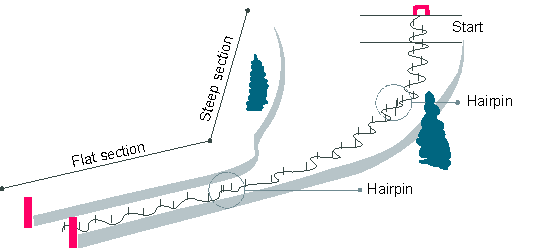
\includegraphics[width=1\linewidth]{figure/figure_introduction_course.pdf}
    \caption{Enter Caption}
    \label{fig: flatcourse}
\end{figure}

\section{How can we improve performance on flats in slalom?}
Now that I have decided to study the flat section of a slalom course, the following question arises: what can skiers do to ski faster on flat terrain in alpine skiing? In alpine skiing, these strategies ultimately revolve around how skiers effectively manage their mechanical energy to achieve desired outcomes \cite{supej_differential_2008, supej_how_2010}. Therefore, in this section, I will outline the fundamental mechanical principles of skiing before proposing four strategies to potentially improve the performance of skiers on flat terrain in slalom.

\subsection{Energy mechanics of alpine skiing}
From a mechanical energy perspective, skiers accumulate gravitational potential energy when they take the ski lift to the top. This acquired potential energy is the skier's primary engine \cite{supej_differential_2008, supej_mechanical_2011} and enables them to do work such as making the ski penetrate the snow to make it turn. The amount of potential energy available to the skier for performing such work at the top of a slalom course can be derived from the following equation:
\[U=mgh\]
Here, $U$ represents the gravitational potential energy (measured in joules), $m$ represents the mass of the skier (measured in kilograms), g represents the gravitational acceleration (approximately $m/s^2$) acting on the skier, and $h$ represents the height (measured in meters). When the skier descends the slalom course, the amount of work done by gravity can be derived by finding the gravitational potential energy for the initial position $U_1$ (e.g., at the top of the slalom course) and the gravitational potential energy for the final position $U_2$ (e.g., at the end of the first turn); then, the negative change in potential energy can be calculated: 
\[W=-U_2 + U_1\]
\[W= -\Delta U \]
This quantity represents the work of gravity on the skiers as they descend from the top to the lower position of the slalom course. According to the law of conservation of mechanical energy, all this work must be converted to kinetic energy when gravity is the sole force acting on the skier. The skiers' kinetic energy can be represented by the following equation:
\[ K = \frac{1}{2} m v^2 \]
where $K$ is the kinetic energy, $m$ is the mass of the skier, and $v$ is the velocity of the skier. Consequently, the sum of the potential and kinetic energy  (denoted as $E$ for mechanical energy) remains constant during a descent, as expressed by the following equation:
\[ E = U + K \]
During descents, however, skiers are exposed to two dissipative forces that oppose motion and can result in some loss of energy transfer to kinetic energy. For skiers, these two dissipative forces are air drag and snow friction (collectively denoted as $D$)\cite{supej_differential_2008}. Therefore, the total mechanical energy during a descent equals the sum of the kinetic energy and the dissipating forces (equation below), and is conceptually illustrated in Fig. \ref{fig:energy}.
\[ U = K + D\]
Consequently, in terms of the mechanical energy principle, a skier's goal during a descent should be to maintain high kinetic energy \cite{supej_differential_2008, supej_mechanical_2011, supej_how_2010}. One way for skiers to achieve this on flat slopes in alpine skiing is by reducing skidding\cite{reid_kinematic_2010, reid_turn_2009}. This can be accomplished by executing carving turns instead of skidding. Most skilled skiers already navigate flat terrains with carving turns, so the question arises whether there are other strategies that can account for the time differences on flats in slaloms and that can be trained to improve race times in flats in slalom.  

\subsection{Strategies to improve race times in flats in slalom}
Here I outline four strategies for potentially improving flat terrain race times, all rooted in the mechanics of energy.

\begin{figure}[H]
\centering
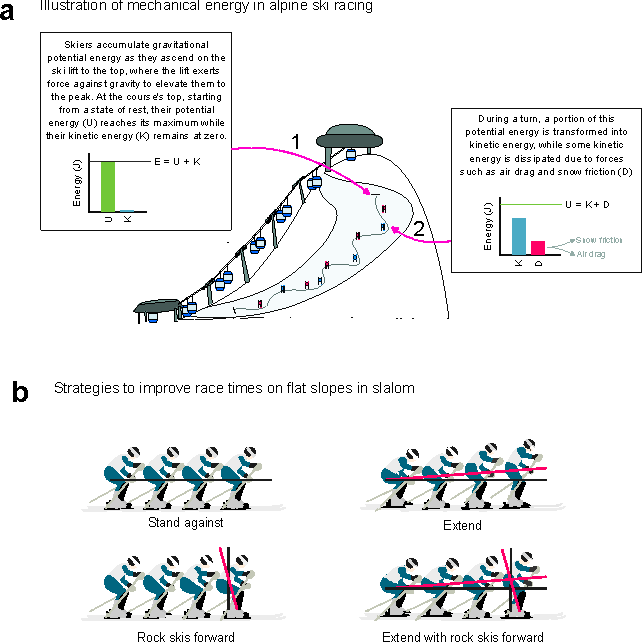
\includegraphics{figure_energymechanics.pdf}
\caption{Kommer}
\label{fig:energy}
\end{figure}

One strategy skiers can exploit to maintain high kinetic energy during a turn and therefore improve their race times on flat sections in slalom is the 'stand against' technique, and is instructed by many ski coaches. In this technique, skiers maintain a stable stance and actively resist being compressed toward their bindings by centrifugal force during a turn (from the skier's frame of reference). According to Lind and Sander's theoretical model on 'pumping to increase velocity' \cite{lind_physics_2013}, this active force resistance could minimize skiers' kinetic energy loss during a slalom turn by keeping the moment of inertia about the axis of rotation fixed instead of increasing it, as would occur if the skier collapsed during the turn. In their model, the rotational kinetic energy of a ski turn can be represented by the following equation: 
\[ T = \frac{L^2}{2I} \]
Here, $T$ represents the kinetic energy of rotation, and $L$ represents the angular momentum (that is, angular velocity ($\omega$) multiplied by the moment of inertia about the axis of rotation ($I = mr^2$)). Lind and Sanders considered a rider traveling on a cart on a friction-free rail with a curved turn and no torque to act on the system. In this situation, if the rider were to collapse toward the cart due to the centrifugal force, the moment of inertia would increase by lengthening the radius about the axis of rotation. Consequently, some rotational kinetic energy is lost if the skier fails to resist the centripetal force. Stand against might therefore be an effective strategy to exploit do ski fast on flats in slalom.  

A second and perhaps better strategy skiers can employ to maintain high kinetic energy during a turn is to 'rock skis forward'. By shifting their vertical position forward and backward, skiers regulate the ski’s total pressure distribution against the snow\cite{lemaster_skiers_1999, lemaster_ultimate_2010, howe_new_2001}. This regulation not only helps skiers maintain balance but also affects the ski's turning behavior. For example, when skiers edge their skis, moving the center of mass toward the tip of the ski increases the pressure distribution on the ski's forebody, enabling it to turn more sharply. Conversely, if skiers edge their skis but shift their center of mass backward to the ski's tail, they decrease the pressure at the ski's forebody and consequently make the turn more gradual \cite{lemaster_skiers_1999, lemaster_ultimate_2010}. In ski racing, skiers generally aim to turn more sharply in the beginning and during the turn and should therefore shift their center of mass to distribute the pressure to the ski's forebody to make it engage with the snow. However, after gate passage, skiers generally aim to stop turning and should therefore shift their center of mass backward by rocking the skis forward. By rocking the skis forward after gate passage, skiers could in principle counteract the unnecessary loss of kinetic energy caused by the skis penetrating and digging unnecessarily into the snow in the exit of the turn. In support of this, previous research has found a strong linear relationship between the skier's forward position and energy dissipation \cite{reid_turn_2009, reid_kinematic_2010}. Additionally, faster skiers have shown to rock their skis more forward and pressure the back part of the ski for considerably longer during a turn compared to slower skiers\cite{reid_kinematic_2010, tjorhom_beskrivelse_2007}. Consequently, rocking skis forward could be an even better strategy than the stand against strategy for improving race times on flat terrain in slalom 

The third strategy that can potentially make skiers faster on flat slopes in slalom is to 'extend,' also referred to as 'pumping' to increase velocity \cite{lind_physics_2013}. When skiers move their center of mass closer to the axis of rotation of a turn from a laterally inclined position by extending their legs, they increase their kinetic rotational energy under certain situations. According to Lind and Sanders \cite{lind_physics_2013} model, the skier achieves this effect by shortening the radius of the axis about which they rotate, which will reduce the moment of inertia and consequently increase the rotational kinetic energy of the system under the assumption that angular momentum is conserved. In their model, the gain in rotational kinetic energy from this motion is proportional to the amount of work the skier does against the centrifugal force (from the skier's frame of reference); therefore, a larger extension movement will accomplish a greater increase in rotational kinetic energy. Scientists have previously assumed that the contribution of pumping to increase the velocity through a turn is minimal and an negotiable mechanism to leverage to improve skiers' race times\cite{supej_differential_2008}. Critics are directed that Lind and Sander's model neglects friction and that it only should work with low speeds \cite{supej_differential_2008, supej_how_2010}. Nevertheless, several studies has been observed that skilled alpine skiers gain additional kinetic energy at the exit of the turn—an increase that cannot be accounted for solely by their available potential energy at that moment\cite{reid_kinematic_2010, supej_how_2010, supej_differential_2008}. Moreover, in an experiment we conducted in 2012, elite skiers had better race times on a flat slalom section when they skied the course with the pumping technique than when they skied the section straight down, despite taking a significant longer trajectory in skiing the course. Therefore, "extend" could be a very important strategy.  

The final strategy is to "extend with rock skis forward", which combines "extend" and "rock skis forward". In a simulation study of skiers pumping on a an undulating terrain, this was the the best performing strategy \cite{mote_accelerations_1983}, and it has been suggested that this could be the best strategy to perform in slalom turns in certain situations \cite{reid_kinematic_2010}. We therefore considered this strategy as the theoretical best strategy. 

Selv om det teori og observasjoner av skikjørere i felt som skulle tilsi at 'extend' and 'extend with rock skis forward' skulle være effektive strategier, finnes det ingen eller lite eksperimentelt arbeid for å estimere effektene av disse strategiene på prestasjoner i flate deler av en slalåmløype. Om pumping gjennom strekking er en effektiv strategi for å kjøre fort på flater, er det også interessant å undersøke de kinematiske endringene i en utøveres skikjøring som følge av en intervensjon på pumping. 


\section{What is the best way to teach these skills?}
Once we have identified which strategies are effective in a particular situation, such as skiing fast on flat slopes in slalom (in our case), our next question is how we should train learners to better learn these strategies? Generelt har skitrenere to main teaching strategies de kan bruke for å oppnå dette i skibakken: de kan instruere og gi feedback til skikjørere og de kan sette løyper. Spørsmålet er om det er mulig å forbedre måten man gir tilbakemelding og instruksjoner på eller setter løyper i forhold til dagens praksis.

\subsection{Can coaches improve their instruction and feedback using reinforcement learning? }
As coaches likely employ various teaching strategies, we exercise caution in generalizing and asserting that all coaches teach in a specific way. Nevertheless, it is quite typical for coaches to use instruction-based teaching in sports\cite{williams_practice_2005, williams_effective_2023, hodges_modelling_2002}. In this approach, they offer performers a correct solution followed by corrective feedback. For instance, a ski coach may encourage the skier to take a shorter line around the gate and then further encourage the learner to shorten the line after a few trials. This teaching strategy can be likened to supervised learning in motor learning, where the difference between the desired strategy and the performer's movement outcome represents a teaching signal for skill improvement  \cite{jordan_forward_1992, wolpert_motor_2010, doya_complementary_2000}. Through practice, this teaching signal can bring the performer closer to executing what is assumed to be the correct choice. But is this teaching strategy truly the most effective approach for enabling learners to select and employ effective strategies? 

Supervised learning offers a promising approach for assisting learners in making informed strategy choices, yet it may also lead learners away from discovering the optimal strategy. First, the coach's advice may not be the optimal solution, as the strategy that coaches believes to be optimal does not always align with reality, even for the best-trained eye \cite{supej_impact_2019, cochrum_visual_2021}. Consequently, learners might be hindered to learn the best strategy when coaches opt for suboptimal strategies \cite{gray_plateaus_2017}. Worse, these learned suboptimal strategies might turn into habits that can be difficult to break \cite{popp_effect_2020}. Second, learners trained through supervised learning might also be constrained to adopting a single ('universal') strategy for all situations rather than acquiring a repertoire of strategies and discerning the most effective strategies for each specific scenario. Finally, it remains uncertain whether the prescriptive approach is the most effective teaching strategy for enabling performers to achieve long-lasting learning effects \cite{wulf_instructions_1997, hodges_role_1999, williams_practice_2005,williams_effective_2023}. 

Another, yet much less frequently adopted, teaching strategy to help learners learn to make good choices is through reinforcement learning \cite{sutton_reinforcement_2018}. The cornerstone of this approach is that the learner learns from evaluations instead of instruction, which occurs by using successes and failures of outcomes as teaching signals. That is, the performer learns the value of different strategies which allows them to finally pick the best solution, rather than being told the putatively correct solution to the problem. Specifically, these values are learned by comparing a given choice's outcomes with the choice's currently expected outcome. Outcomes that exceed or fall short of expectations result in errors in reward prediction, signaling that the learner must update their predictions to better anticipate future rewards following that action \cite{rescorla_theory_1972}. These reward prediction errors are then incorporated to form a new and better estimate of expected reward by updating expectations through a weighted running average. The computations underlying this form of value-learning of choices have been tremendously powerful in explaining human and animal learning \cite{waelti_dopamine_2001, schultz_neural_1997, pessiglione_dopamine-dependent_2006,lee_neural_2012, law_reinforcement_2009} as well as training AI to perform complex tasks such as computer games starting from pixel inputs, only\cite{mnih_human-level_2015}. In addition, reinforcement learning has been shown to improve motor skill learning on simple tasks performed in the laboratory \cite{lior_shmuelof_overcoming_2012, abe_reward_2011, truong_error-based_2023, hasson_reinforcement_2015}. Based on this evidence, we ask whether reinforcement learning offers a better alternative for training learners to make better decisions about strategies than traditional supervised learning with a coach. 


\subsection{Can coaches improve course setting using the contextual interference effect}
Den andre teaching strategy som skitrenere kan bruke for å oppnå læring er gjennom løypesetting. Gjennom løypesetting forandrer man oppgaven som utøvere blir satt til å løse. Setter trenere for eksempel en løype med mye sving krever de en lavere turn radius enn hvis de setter en løype med lavere sving. Trenerens løypestikk kan ha forskjellige funksjoner som å reduksjon av skader. Because skiers never know what courses to expect in a race, they must master an extensive range of cpurses. Therefore, undertaking training to perfect performance in a single course setting may not be effective. Spørsmålet er om man kan oppnå bedre læring gjennom smartere måter å bruke løypesetting på?

One method to potentially achieve this goal is to train slalom courses with large contextual interference. This teaching strategy involves training tasks (in our case courses) in a nonrepetitive sequence (that is, interleaved order), such as practicing tasks A, B, and C in the order of BCA, ACB, or ABC, rather than a practice structure where tasks are repeated in blocks (that is, blocked practice), such as AAA, BBB, or CCC. This nonsystematic training structure has been shown to be an effective teaching strategy for improving skill retention and transfer in various simple learning tasks.

Two main explanations have been proposed to account for the contextual interference effect: the elaboration hypothesis and the reconstruction/forgetting hypothesis. The elaboration hypothesis proposes that interleaved practices prompt individuals to process information more eloborately during acquisition, which enriches their understanding and problem solving techniques. This increased elaboration process enhances retention, which is not fully realized when practicing tasks in a blocked order. In contrast, the reconstruction/forgetting hypothesis posits that increased task switching provides more opportunities to forget task-relevant information held in working memory. This forgetting of task-relevant information forces the learner to reconstruct the action plan for every trial the learner revists the task. The repetitive process of abandoning and reconstructing action plans during interleaved practice contributes to better memory formation and thus increased retention.

The contextual interference effect has not always succeeded in transferring to the learning of real-world skills, however. This discrepancy can be understood through the challenge-point framework, where the effect of contextual interference is moderated by both the difficulty of the task and the skill level of the performer. In this framework, easy tasks can benefit from contextual interference to make the task more challenging, whereas difficult tasks are already challenging enough to serve as adequate learning stimuli on their own and are best learned without contextual interference initially. As the learner becomes more skilled, the learning process may benefit from increased contextual interference to improve the level of difficulty. In align with this prediction, studies have shown that beginners who learn skills when practice increases from blocked to interleaved practice learn better than those who use blocked or interleaved practice alone. 

One derived prediction from the challenge point framework is that skilled performers can benefit from interleaved practice to make training more challenging and therefore better. Consistent with this notion, Hall found that skilled baseball players who practiced batting achieved better retention through interleaved practice compared to blocked practice. I motsetning til dette resultatet fant ingen statistically significant differences in retention were not found between tennis players learning to serve in three different ways through interleaved practice and blocked practice. Instead, these researchers found evidence for improved transfer to a new situation. Thus, it is not entirely clear whether contextual interference can be generalized to skilled performers. One idea is that contextual interference is more beneficial in open sports where performers must constantly switch between different strategies to solve tasks, thereby potentially being important for alpine skiers. An important aim of the study was thus to investigate whether the contextual interference effect can be used to improve the training of skilled performers. 



%For example, \href{https://www.frontiersin.org/articles/10.3389/fbioe.2022.966041/full\#B2}{Barreiros et al. (2007)} have reported that the proportion of studies showing improved retention due to interleaved practice was considerably smaller for skills performed in a natural environment than for skills performed in a laboratory environment.






%Despite the existence of ample evidence for the contextual interference effect being present in laboratory environments, it has become clear that the principles deriving from the research do not always generalize to the learning of motor skills in naturalistic settings such as sports (\href{https://www.frontiersin.org/articles/10.3389/fbioe.2022.966041/full\#B52}{Wulf and Shea, 2002}; \href{https://www.frontiersin.org/articles/10.3389/fbioe.2022.966041/full\#B5}{Brady, 2004}; \href{https://www.frontiersin.org/articles/10.3389/fbioe.2022.966041/full\#B2}{Barreiros et al., 2007}). For example, \href{https://www.frontiersin.org/articles/10.3389/fbioe.2022.966041/full\#B2}{Barreiros et al. (2007)} have reported that the proportion of studies showing improved retention due to interleaved practice was considerably smaller for skills performed in a natural environment than for skills performed in a laboratory environment. Furthermore, a meta-analysis showed that the contextual interference effect is typically smaller and more dispersed than in laboratory tasks (\href{https://www.frontiersin.org/articles/10.3389/fbioe.2022.966041/full\#B5}{Brady, 2004}). Therefore, while interleaved practices may improve learning for simple tasks, the evidence for contextual interference for learning more complex tasks in natural environments is not conclusive. 









 



%To forklaringer foreslått for denne effekten er the elaboration hypothesis and the reconstruction/forgetting hypothesis. Den første av disse forklaringene er at den hyppig oppgavebyttingen i interleaved practice gjør at man prosesserer informasjon med ulike innganger, som beriker hvordan man forstår og løser oppgaven. Denne økte elaboration prosessen forbedrer retention. Dette oppnår man ikke like fullt om man trener oppgavene blocked. I kontrast mener rekonstruering/forgetting hypotesen at den hyppige oppgavebyttingen fører til 'glemsel' ved at oppgavebyttet skaper et brudd i læringen, som gjør at en aktiv handlingsplan må forlates og erstattes med en annen. Den gjentagende prosessen med å forlate og gjenoppta minnet bidrar til bedre minnedannelse og dermed økt retention. 



%To achieve this goal, ski coaches have two main teaching strategies at their disposal: one involves how they instruct and give feedback on the strategies, and the other involves how they set up slalom courses to create situations in which these strategies can be learned. In the order of how coaches normally plan and organize training sessions, the first step of any session is to determine which strategies to prioritize and instruct. Once these strategies are determined, the coach proceeds to set up a slalom course on the terrain with appropriate dimensions suitable for practicing these strategies. Since the race regulations allow for many different course layouts, the race courses vary greatly. Therefore, an important element in training is to ensure that the course setting is not too narrow, so that skiers learn to perfect the skill not only for one or a few situations but also for the wide range of variations that occur in competition. After the course is set, the coach's role is to provide instruction and feedback on the skiers' race performance and, if necessary, adjust the course setting on the fly to make it easier or harder for the skiers to execute the strategy. 

%Hvordan trenere setter løype i dag er for mange trenere noe de setter på rutine, som lett utvikler seg til habits ved gjentakende. Generelt kan vi si at de utvikler en typisk fingeravtrykk på deres løypesetting som de. Utfordringen med dette er at vi får utøvere som ikke ser klarer å tilpasse strategiene så godt til andre situasjoner. Skaderisiko, 

%In contemporary teaching practice, performers commonly learn which movement strategy to execute with instruction-based teaching. That is, a coach or teacher advises the performer 'what to do' (e.g., suggesting taking a shorter line around the gate) followed by corrective feedback (e.g., encouraging the learner to further shorten the line) \cite{williams_practice_2005, williams_effective_2023, hodges_modelling_2002}. This teaching strategy can be likened to supervised learning in motor learning, where the difference between the desired strategy and the performer's movement outcome represents a teaching signal for skill improvement  \cite{jordan_forward_1992, wolpert_motor_2010, doya_complementary_2000}. Through practice, this teaching signal can bring the performer closer to executing what is assumed to be the correct choice. But is this teaching strategy truly the most effective approach for enabling learners to select and employ effective strategies? 

%Although supervised learning serves as a reasonable approach to improve performers' strategies, the teaching strategy has limitations that may prevent performers from converging on an optimal strategy. First, the coach's advice may not be the optimal solution, as what coaches judge as a good strategy does not always align with reality, even for the best-trained eye \cite{supej_impact_2019, cochrum_visual_2021}. Performers might therefore miss opportunities to discover the best strategy when coaches opt for suboptimal strategies \cite{gray_plateaus_2017}. Worse, these learned suboptimal strategies might turn into habits that can be difficult to break \cite{popp_effect_2020}. Second, performers trained through supervised learning might also be constrained to adopting a single ('universal') strategy for all situations rather than acquiring a repertoire of strategies and discerning the most effective strategies for each specific scenario. Finally, it remains uncertain whether the prescriptive approach is the most effective teaching strategy for enabling performers to achieve long-lasting learning effects \cite{wulf_instructions_1997, hodges_role_1999, williams_practice_2005,williams_effective_2023}. 


%A key question is whether coaches can improve the way they instruct, provide feedback, and set slalom courses by applying principles from cognitive science? In the following paragraphs, I will first delve into what skill level and expertise development entail before introducing two key learning principles from cognitive science that could potentially improve coaches' approaches. 





%\subsection{What is motor skill learning?}
%Vi har ofte lite utfordring med å identifisere en god prestasjon når vi ser det. For eksempel kan vi si at en alpinist som kjører rene og raske svinger ned et bratt og isete heng i slalåm for å være skilled. Til tross for dette, klarer ikke forskere å enes om en bestemt definisjon hva det er. Noen forskere har heller forsøkt å snevre inn motor skill learning ved å eksludere hva det ikke er. Ved å gjøre det snakker man ofte om at skilled performance er å utføre en bevegelse snarere enn å kommunisere hva man kan fortelle om ferdigheten. Man skiller også motor skill learning fra adaptasjonsprosesser som ofte blir tilbakestilt med en gang. På et overordnet nivå dreier motorisk læring seg om å successfully achieve goals. Når dette er snakk om motorisk handlinger, snakker vi om motorisk utførelse.

%Forskere har på en annen side begynt å lande på hvilke komponenter som inngår i ferdighetslæring. På den ene siden handler det om å velge gode strategier (action selection). For eksempel må en alpinist bestemme seg for om man skal velge en lang linje eller kort linje ned i fart. Når denne strategien er valgt er det viktig at denne handlingen utføres så presist og godt som mulig (action execution). Til slutt er det viktig at disse handlingene utføres så presist som mulig. 

%Et kanskje tredje element er å velge gode strategier. Kanskje si noe om de læringmekanismene som støtter dette. 


%- Multiple learning mechanism

%Many studies suggest that training with a high degree of contextual interference can create favorable conditions for learning motor skills (\href{https://www.frontiersin.org/articles/10.3389/fbioe.2022.966041/full\#B28}{Magill and Hall, 1990}; \href{https://www.frontiersin.org/articles/10.3389/fbioe.2022.966041/full\#B23}{Lee and Simon, 2004}; \href{https://www.frontiersin.org/articles/10.3389/fbioe.2022.966041/full\#B29}{Merbah and Meulemans, 2011}). Experiments on the contextual interference effect usually introduce learners to three tasks to be learned (tasks A, B, and C). In the high contextual interference condition (i.e., interleaved practice), the practice order of tasks makes the learner frequently switch between the tasks they acquire (for example, ABC, BAC, or CBA). In contrast, less switching occurs in the low contextual interference condition (i.e., blocked practice) by arranging the tasks in blocks (for example, AAA, CCC, BBB). Previous research has provided evidence that interleaved practice often improves skill preservation over time (i.e., retention) and adaptation of the skill to new situations (i.e., transfer) compared to blocked practice. However, a notable aspect is that blocked practice often results in superior performance during skill acquisition compared to the interleaved group. This paradoxical interaction—called the contextual interference effect—represents a prime example of the distinction between performance and learning in motor learning and has been extensively replicated in a wide variety of scientific laboratory experiments (\href{https://www.frontiersin.org/articles/10.3389/fbioe.2022.966041/full\#B40}{Shea and Morgan, 1979}; \href{https://www.frontiersin.org/articles/10.3389/fbioe.2022.966041/full\#B22}{Lee and Magill, 1983}; \href{https://www.frontiersin.org/articles/10.3389/fbioe.2022.966041/full\#B41}{Simon and Bjork, 2001}; \href{https://www.frontiersin.org/articles/10.3389/fbioe.2022.966041/full\#B47}{Thomas et al., 2021}).

%Despite the existence of ample evidence for the contextual interference effect being present in laboratory environments, it has become clear that the principles deriving from the research do not always generalize to the learning of motor skills in naturalistic settings such as sports (\href{https://www.frontiersin.org/articles/10.3389/fbioe.2022.966041/full\#B52}{Wulf and Shea, 2002}; \href{https://www.frontiersin.org/articles/10.3389/fbioe.2022.966041/full\#B5}{Brady, 2004}; \href{https://www.frontiersin.org/articles/10.3389/fbioe.2022.966041/full\#B2}{Barreiros et al., 2007}). For example, \href{https://www.frontiersin.org/articles/10.3389/fbioe.2022.966041/full\#B2}{Barreiros et al. (2007)} have reported that the proportion of studies showing improved retention due to interleaved practice was considerably smaller for skills performed in a natural environment than for skills performed in a laboratory environment. Furthermore, a meta-analysis showed that the contextual interference effect is typically smaller and more dispersed than in laboratory tasks (\href{https://www.frontiersin.org/articles/10.3389/fbioe.2022.966041/full\#B5}{Brady, 2004}). Therefore, while interleaved practices may improve learning for simple tasks, the evidence for contextual interference for learning more complex tasks in natural environments is not conclusive.

%Over the years, researchers have proposed and examined several different moderators to account for the contradictory results between laboratory and natural environments, including the learner’s age (\href{https://www.frontiersin.org/articles/10.3389/fbioe.2022.966041/full\#B8}{Del Rey et al., 1983}), the amount of practice (\href{https://www.frontiersin.org/articles/10.3389/fbioe.2022.966041/full\#B39}{Shea et al., 1990}), the type of task (\href{https://www.frontiersin.org/articles/10.3389/fbioe.2022.966041/full\#B28}{Magill and Hall, 1990}), the modality-specific requirements of the task (\href{https://www.frontiersin.org/articles/10.3389/fbioe.2022.966041/full\#B38}{Schöllhorn et al., 2022}), and the learner’s skill level relative to the difficulty of the task (\href{https://www.frontiersin.org/articles/10.3389/fbioe.2022.966041/full\#B52}{Wulf and Shea, 2002}; \href{https://www.frontiersin.org/articles/10.3389/fbioe.2022.966041/full\#B16}{Guadagnoli and Lee, 2004}). Concerning the latter of these moderators, the challenge-point framework (\href{https://www.frontiersin.org/articles/10.3389/fbioe.2022.966041/full\#B16}{Guadagnoli and Lee, 2004}) posits that the efficacy of interleaved practice depends on the difficulty of the task as it is objectively defined (that is, nominal task difficulty) but also how challenging the task is relative to the learner’s skill level and practice environment (that is, functional task difficulty). The framework predicts that an interleaved practice may be more beneficial to promoting learning in a context involving learning a task with low nominal difficulty (for example, a simple laboratory task). This expected observation is because interleaved practice increases the functional difficulty of the task to engage the cognitive mechanisms responsible for causing the contextual effect. With more nominally difficult tasks, the task’s characteristic may already be sufficiently challenging to achieve this end so that beginners may benefit from the blocked practice. However, as learners become better at the task, increasing the functional difficulty of the task through interleaved practice may be needed to engage the cognitive mechanisms to promote additive learning. In support of the challenge-point framework, several studies have provided evidence that providing beginners with a gradual and systematic increase in contextual interference when learning complex skills seem to be a better learning approach than the sole use of blocked or interleaved practice (\href{https://www.frontiersin.org/articles/10.3389/fbioe.2022.966041/full\#B32}{Porter and Magill, 2010}; \href{https://www.frontiersin.org/articles/10.3389/fbioe.2022.966041/full\#B36}{Saemi et al., 2012}). These findings suggest that the optimal practice condition changes with the learner’s proficiency and the skill’s complexity.

%The challenge point framework and the supporting evidence that the learner’s skill level interacts with the characteristic of the task in determining the contextual interference effect can build the impression that skilled performers benefit from training with a high degree of contextual interference when improving or refining their skills. Even though some researchers have advocated such an approach (\href{https://www.frontiersin.org/articles/10.3389/fbioe.2022.966041/full\#B7}{Christina and Bjork, 1991}; \href{https://www.frontiersin.org/articles/10.3389/fbioe.2022.966041/full\#B37}{Schmidt, 1991}), few studies have explicitly tested it. One of the few exceptions is a study on skilled baseball players who performed additional batting training to probe the contextual interference effect (\href{https://www.frontiersin.org/articles/10.3389/fbioe.2022.966041/full\#B17}{Hall et al., 1994}). Three groups practiced batting with three types of baseball pitches. The blocked group practiced these pitches in a blocked order (AAA, BBB, CCC), whereas the interleaved group practiced them in a random order (BCA, ABC, BAC). At the end of the training intervention, the interleaved group performed better than the blocked group. This study demonstrated that interleaved practice might also improve learning for skilled performers. It is important to note that \href{https://www.frontiersin.org/articles/10.3389/fbioe.2022.966041/full\#B17}{Hall et al. (1994)} used variations of a single skill (i.e., batting) to probe the contextual interference effect. In a recent study, \href{https://www.frontiersin.org/articles/10.3389/fbioe.2022.966041/full\#B6}{Buszard et al. (2017)} performed a between-skill manipulation to examine the contextual interference effect in youth tennis players. While interleaving the practice schedule did not improve retention for these players compared to the blocked practice schedule on the same task, there was evidence that the interleaved group transferred their skill better to competition (i.e., transfer). Hence, it remains unclear whether training with contextual interference improves learning for skilled performers when improving their skills. This lack of understanding is critical to address in order to provide proper recommendations for instructors in sports and other motor activities, such as surgical operations in medicine and the training of military personnel.

%Testing the contextual interference effect on skilled performers implies specific challenges that must be overcome and effectively solved. The biggest challenge is that skilled performers are usually obsessed with achieving success in their activity and devote significant amounts of their time and resources to improving their performance in this activity. Therefore, recruiting them for a study is often challenging because of their reluctance to modify their training for an experiment, especially if it does not lead to immediate performance gains (\href{https://www.frontiersin.org/articles/10.3389/fbioe.2022.966041/full\#B10}{Farrow and Buszard, 2017}). Even if performers were willing to participate, it would often require a large volume of practice to improve the performance of a skilled practitioner compared to a novice performer (\href{https://www.frontiersin.org/articles/10.3389/fbioe.2022.966041/full\#B17}{Hall et al., 1994}). Hence, even if interleaved practice makes the training more effective, the effect may only become visible after extensive practice, regardless of the skills training method. A final obstacle is that it is often difficult to achieve a robust and sensitive performance goal, especially in alpine ski racing, where external conditions such as snow and wind vary considerably and may influence performance (\href{https://www.frontiersin.org/articles/10.3389/fbioe.2022.966041/full\#B50}{Williams et al., 2017}). Overcoming these challenges requires in-depth knowledge of the skill domain, and real-world practitioner skills are needed to invent innovative approaches to assess skills and deal with issues of validity at the same time (\href{https://www.frontiersin.org/articles/10.3389/fbioe.2022.966041/full\#B10}{Farrow and Buszard, 2017}).

%Considering the need for a better understanding of how the contextual interference effect translates to skilled learners, and how to cope with the described challenges, we have investigated the contextual interference effect on skilled athletes in the complex sport of alpine ski racing in this study. Alpine ski racing is a sport where performance is measured as the time from start to finish, where athletes need to pass through a pre-defined course marked with gates. The sport consists of six main disciplines: slalom (SL), giant-slalom (GS), super-G (SG), downhill (DH), Parallel and Combined, which vary in the number of direction changes,timing and dynamics in turns,terrain and transitions, course length, and jumps (\href{https://www.frontiersin.org/articles/10.3389/fbioe.2022.966041/full\#B15}{Gilgien et al., 2018}). Of these six disciplines, slalom skiing is the most technically demanding due to its frequent changes of direction, high turn forces, and small turn radii (\href{https://www.frontiersin.org/articles/10.3389/fbioe.2022.966041/full\#B35}{Reid, 2010}). Slalom courses generally comprise ∼50 gates, adjacently positioned with a linear distance of 6–13 m. These courses can vary extensively between races depending on the course setter, usually a coach who can determine the type of course within the rules of Fédération International de Ski (FIS). Besides the variability in courses, there is also large variability in terrain characteristics (for example, incline and terrain transitions), snow properties, and weather (for example, visibility). Slalom racers should therefore expect a significant degree of variability in conditions in the performance arena.

%Although the total time differences between skiers in slalom races can be quite small, section differences through a course can be quite significant while typically equalizing to small differences at the finish (\href{https://www.frontiersin.org/articles/10.3389/fbioe.2022.966041/full\#B44}{Supej and Cernigoj, 2006}; \href{https://www.frontiersin.org/articles/10.3389/fbioe.2022.966041/full\#B46}{Supej and Holmberg, 2011}). The sections of slalom courses where significant time differences typically occur between skiers are flat terrain sections (\href{https://www.frontiersin.org/articles/10.3389/fbioe.2022.966041/full\#B44}{Supej and Cernigoj, 2006}). An essential characteristic of flat sections is that the component of gravity that accelerates the skiers downhill is small (\href{https://www.frontiersin.org/articles/10.3389/fbioe.2022.966041/full\#B35}{Reid, 2010}). Therefore, the skier must make the necessary adjustments to their technique to ski fast in this type of terrain (\href{https://www.frontiersin.org/articles/10.3389/fbioe.2022.966041/full\#B45}{Supej et al., 2015}). One technique proposed to help increase speed in flat terrain is to “pump” while turning to increase the turn exit speed (\href{https://www.frontiersin.org/articles/10.3389/fbioe.2022.966041/full\#B30}{Mote and Louie, 1983}; \href{https://www.frontiersin.org/articles/10.3389/fbioe.2022.966041/full\#B25}{Lind and Sanders, 2004}). In this context, pumping refers to the technique of extending the legs and pushing the center of mass towards the axis of rotation at the center of the turn. Through the conservation of angular momentum, pushing the center of mass closer to the axis of rotation can lead to increased tangential velocity (\href{https://www.frontiersin.org/articles/10.3389/fbioe.2022.966041/full\#B25}{Lind and Sanders, 2004}). Therefore, the extent and quality with which skiers can exploit this technique can be a primary explanation for the time differences in flat sections.

%Because the technique that leads to good performance differs depending on the terrain incline, researchers have recommended dividing training into sessions with uniform terrain inclines to achieve more element-focused training (\href{https://www.frontiersin.org/articles/10.3389/fbioe.2022.966041/full\#B45}{Supej et al., 2015}). Once training in a section of uniform terrain incline, coaches need to determine the slalom gates’ location down the hill. The location of the gates determines two characteristics of the course: the linear distance between successive gates determines the room skiers have for turning between gates, and the offset determines how “turny” the course is. Changes in these two course dimensions can cause significant changes in the required technique, and the tactics skiers must use to ski the course. For example, changes in gate offset have been shown to reduce speed and turn radius but increase turn forces, impulse (a measure of physical load), and inward lean for giant slalom and super-G (\href{https://www.frontiersin.org/articles/10.3389/fbioe.2022.966041/full\#B43}{Spörri et al., 2012}; \href{https://www.frontiersin.org/articles/10.3389/fbioe.2022.966041/full\#B13}{Gilgien et al., 2020}, \href{https://www.frontiersin.org/articles/10.3389/fbioe.2022.966041/full\#B12}{Gilgien et al., 2021}). In contrast, shortening the linear distance between gates causes a reduction in turn time and speed but has a limited effect on forces and turn radii compared to changes in the offset (\href{https://www.frontiersin.org/articles/10.3389/fbioe.2022.966041/full\#B35}{Reid, 2010}; \href{https://www.frontiersin.org/articles/10.3389/fbioe.2022.966041/full\#B13}{Gilgien et al., 2020}, \href{https://www.frontiersin.org/articles/10.3389/fbioe.2022.966041/full\#B12}{2021}). Because course setting has a significant impact on skiers’ technique and is the training variable that coaches can influence the most, there is a general conception that this is one of the most critical variables affecting learning.

%Because skiers never know what courses and conditions to expect in a race, they must master an extensive range of conditions. Therefore, undertaking training to perfect performance in a single course setting may not be effective. Instead, researchers have argued that a better approach is to use interleaved practice in these types of open sports (\href{https://www.frontiersin.org/articles/10.3389/fbioe.2022.966041/full\#B10}{Farrow and Buszard, 2017}). However, few studies have tested this recommendation due to the described challenges of conducting studies on complex learning tasks with skilled performers. Therefore, we established this study to test the contextual interference effect with skilled alpine ski racers in a realistic real-world ski racing environment. An important goal was to do the study with a large number of participants to estimate the contextual interference effect robustly. To achieve this goal, we designed a study that targeted a particular skill element of skiing performance that was relevant for the skiers to improve. Targeting this specific element instead of providing holistic training, we were also able to improve the skiers’ performance by a significant degree, because training this skill was novel for the participants.

%In this study, we expected contextual interference to apply to the training of alpine ski racers. Our rationale for expecting an extension of the effect to this context emerged from previous studies that reported improved retention of continuous skills (cyclic bimanual coordination task) resulting from interleaved compared to blocked practice (\href{https://www.frontiersin.org/articles/10.3389/fbioe.2022.966041/full\#B48}{Tsutsui et al., 1998}; \href{https://www.frontiersin.org/articles/10.3389/fbioe.2022.966041/full\#B31}{Pauwels et al., 2014}). Moreover, in a snow environment, \href{https://www.frontiersin.org/articles/10.3389/fbioe.2022.966041/full\#B42}{Smith (2002)} reported that novices learned snowboarding turns better after practicing four different turns (left/right and heel/toe) in an interleaved compared to a blocked order. This finding suggests that contextual interference may be relevant for learning skills in alpine ski racing. If skiers vary their turns in an interleaved manner, as is accomplished by frequently switching between courses, we could expect to observe contextual interference in alpine skiing. In the snowboarding study, however, the participants were novices, and it is unclear how this extrapolates to skilled performers. Based on the previous research that has provided evidence for the contextual interference for experienced performers (\href{https://www.frontiersin.org/articles/10.3389/fbioe.2022.966041/full\#B17}{Hall et al., 1994}), we hypothesized that interleaved practice would suppress performance during acquisition but improve performance at retention.

 



%What can coaches do to train deliberate practice?






%I den siste fasen forsøker man å finne ut hvordan eksperter tilegner seg ferdighetene for å kjøre for på flater. 


%Deliberate practice and strategies

%Adaptive and skilful

%I





%et viktig innsikt er at. et viktig innsikt ermed hvordan de presterer bedre. er de


%- Tilrettelegging og veiledning


%Organisation, Instruction and feedback

